\section{Platforma iOS}
\subsection{Systémová architektura}
Operační systém iOS vyvíjený společností Apple je založen na jádře Darwin, které je odvozeno z UNIXu \cite{kernel_ios}. Darwin je nejen základem systému iOS, ale i jeho robustnějšího bratra Mac OS X, jenž slouží jako operační systém pro stolní a přenosné počítače firmy Apple. Jádro systému Darwin obsahuje XNU kernel, který je kombinací mikrokernelu Mach s některými prvky systému FreeBSD, které byly přidány zejména kvůli lepšímu výkonu \cite{what_is_darwin}.

iOS podporuje architekturu ARM (konkrétně ARMv6, ARMv7 \cite{bp_dominik}). Na ní postavené čipy dnes pohánějí drtivou většinu smartphonů, tabletů a dalších „chytrých“ přenosných zařízení.

Systém iOS se v zásadě neliší od jiných operačních systémů. Slouží jako most mezi uživatelskými aplikacemi a hardwarem samotného zařízení. Samotné aplikace tak nekomunikují s hardwarem přímo, ale přes abstraktní systémová volání definovaná operačním systémem. Architektura systému iOS se dá rozdělit do čtyř vrstev, jak vidíme na obrázku \ref{fig:iOSSystemLayers} níže. 

\begin{enumerate}
	\item Cocoa Touch – Jedná se o sadu objektově orientovaných frameworků vytvořených za účelem vývojářsky přívětivého vývoje mobilních aplikací. Celá řada postupů a technik je společná s vývojem aplikací pro desktop, avšak Cocoa Touch byla vyvinuta se zaměřením na vývoj pro dotyková zařízení. Cocoa Touch obsahuje celou řadu zajímavých frameworků, z těch známějších můžeme jmenovat například UIKit, jenž se stará především o zobrazování grafických prvků a práci s nimi, MapKit, pomocí nějž můžete do své aplikace implementovat práci s mapami, a mnohé další \cite{bp_dominik}.
	\item Media – Jak již název napovídá, ve vrstvě Media se nachází knihovny pro práci s grafikou, zvukem, videem a podobně.
	\item Core Services – Toto je poslední vrstva, která odděluje vyšší vrstvy od samotného operačního systému. Obsahuje velmi důležité funkce pro práci se systémovými službami.
	\item Core OS – Nejnižší vrstva systému iOS zajišťuje práci s hardwarem. Obsahuje například bezpečnostní framework Security či základní systémová volání (POSIX vlákna, přístup do filesystému, alokace paměti apod.).
\end{enumerate}

\begin{figure}\centering
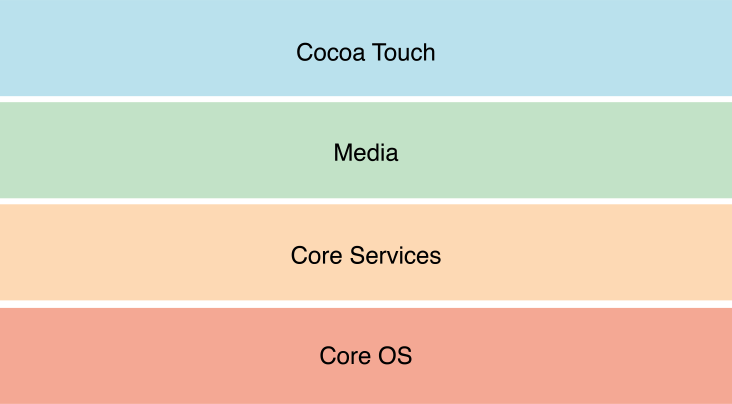
\includegraphics[width=1.0\textwidth]{iOS_SystemLayers.png}
\caption{Platforma iOS, systémové vrstvy \cite{ios_technology_overview}}
\label{fig:iOSSystemLayers}
\end{figure}

Vývojářům je obecně doporučováno využívat co nejvíce technologií z vyšších vrstev této architektury, neboť se jedná o objektové zabstraktnění nízkoúrovňových konceptů.

\subsection{Aplikační technologie}
O celý postprocesing a slinkování hotové aplikace se v iOS starají LLVM (Low Level Virtual Machine) a frontend Clang \cite{bp_dominik}. 

LLVM je kompilátorová infrastruktura pro „Compile Time“, „Link Time“ a „Run Time“, jejíž infrastruktura se dělí na front-end a back-end. Úkolem front-endu je vygenerování bytecodu srozumitelného pro back-end. Back-end následně bytecode zkompiluje do nativního strojového kódu \cite{bp_dominik}. 

Cang je front-end kompilátor pro céčkové programovací jazyky. V našem případě se používá především pro kompilaci jazyka Objective-C o němž si povíme později.

\subsection{Vývojářské technologie}
Aplikace pro systém iOS se programují primárně v jazyce Objective-C \cite{introduction_ios_development}. Objective-C je objektově orientovaný, reflektivní jazyk, v němž lze nalézt společné rysy se známým jazykem SmallTalk \cite{bp_dominik}. Poměrně složitá syntaxe Objective-C představuje značnou překážku pro začínající vývojáře, protože se výrazně liší od ostatních běžně používaných jazyků (například Javy v Androidu).

Díky kompilační struktuře naznačené v předchozí kapitole můžeme však místo Objective-C použít alternativní programovací jazyky, pokud k nim najdeme vhodný front-end. Toho využívá například projekt Monotouch, který vám umožňuje programovat nativní aplikace v C\# a frameworku .NET \cite{xamarin_monotouch}.

\subsection{Vývojářské nástroje}
Apple dává vývojářům k dispozici balík iOS SDK, který obsahuje široké spektrum nástrojů potřebných k tvorbě nativních aplikací pro systém iOS. Tento balík obsahuje například vývojové prostředí XCode, emulátor pro simulovaný běh aplikací na virtuálním zařízení, nástroj pro designování grafických prvků navrhované aplikace, offline verzi dokumentace a mnoho dalšího.

Pro vývoj aplikací pro iOS je nutné vlastnit počítač s operačním systémem Mac OS X. Toto je další poměrně značná překážka pro začínající vývojáře neboť počítače s tímto systémem jsou prozatím na trhu zastoupeny v marginální míře a konkurence v podobě Androidu umožňuje vyvíjet aplikace pro tento systém na libovolné platformě.  Pro publikování aplikací v tržišti App Store je navíc potřeba vlastnit placený vývojářský účet \cite{distribute_ios_app}.

\section{Platforma Android}
\subsection{Systémová architektura}
Architektura operačního systému Android je rovněž vrstevnatá. Jak vidíme na obrázku \ref{fig:AndroidArchitecture}, nejníže se nachází jádro, které se stará o přímou komunikaci s hardwarem zařízení. Android používá jádro Linux verze 2.6, které Google upravil k obrazu svému \cite{android_architecture}. Toto jádro obsahuje ovladače k jednotlivým součástem hardwaru, jako je například fotoaparát, baterie, SD karta a podobně. Zároveň poskytuje vyšším vrstvám rozhraní, pomocí kterého může vývojář hardwarové funkce využít ve svých aplikacích. Android využívá Linux i pro další životně důležité systémové funkce jako je správa pamětí, management procesů, zabezpečení apod.

Nad jádrem leží vrstva knihoven. Tyto knihovny slouží pro práci s různými datovými strukturami a jsou modifikovány zařízení od zařízení. Knihovny jsou napsány v jazyce C či C++. Mezi těmi nejzajímavějšími můžeme zmínit například knihovnu pro práci s databází SQLite či jádro Webkit, jehož prací je správné zobrazování HTML souborů.

Další vrstvou je tzv. Application framework. S tou přijde vývojář do styku nejvíce, neboť zde se nachází většina volání, kterých bude ve svých aplikacích využívat. Application framework se sestává z tzv. bloků, přičemž každý jeden blok slouží k jinému účelu. Za zmínku stojí například Telephony manager, který se stará o správu telefonních hovorů. Můžeme tohoto bloku využít, pokud budeme chtít uživateli umožnit telefonování přímo z aplikace. Neméně důležitý je také Location Manager, jehož úkolem je zjišťování polohy zařízení především pomocí GPS modulu.

Nejvýše v celé hierarchii se nachází vrstva se samotnými aplikacemi. V této vrstvě se vyskytují, krom systémových aplikací jako je Home screen či Kontakty, i uživatelské aplikace.

\begin{figure}\centering
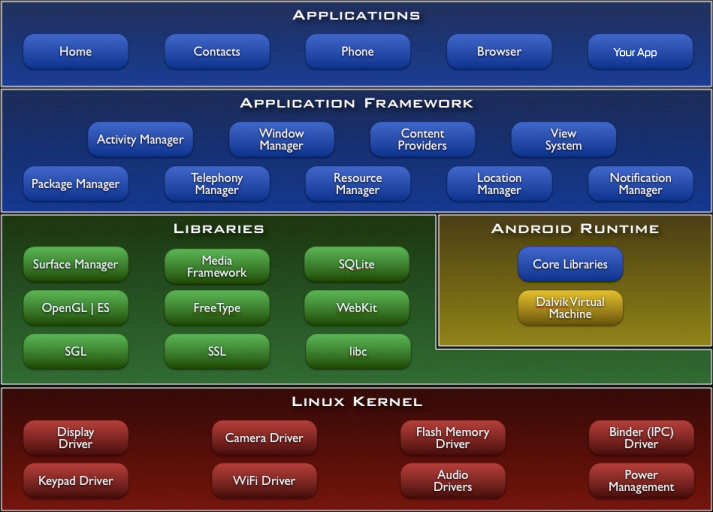
\includegraphics[width=1.0\textwidth]{Android-architecture.jpg}
\caption{Architektura systému Android \cite{android_architecture}}
\label{fig:AndroidArchitecture}
\end{figure}

\subsection{Aplikační technologie}
Nativní aplikace běží ve virtuálním prostředí zvaném Dalvik Virtual Machine. Jedná se o open-source variantu známější Java Virtual Machine, nicméně DVM je speciálně uzpůsobena pro běh na méně výkonných zařízeních, jako jsou právě mobilní telefony \cite{android_architecture}. Každá aplikace běží v instanci tohoto DVM a celá tato instance běží uvnitř Linuxového procesu, který komunikuje přímo s jádrem \cite{introduction_android_development}.

\begin{figure}\centering
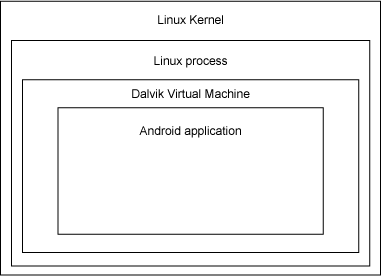
\includegraphics[width=0.6\textwidth]{android_app_tech.png}
\caption{Architektura systému Android 2 \cite{introduction_android_development}}
\label{fig:AndroidArchitecture2}
\end{figure}

\subsection{Vývojářské technologie}
Pro vývoj nativních aplikací se používá programovací jazyk Java. Podle společnosti TIOBE se jedná o druhý nejpoužívanější programovací jazyk na světě \cite{tiobe_software}. Java je objektově orientovaný jazyk se syntaxí blízkou jazykům C a C++.

Velkou výhodou Javy je její platformní nezávislost. Vlastní kód se totiž překládá do tzv. mezikódu, který je poté interpretován v rámci Java Virtual Machine \cite{understanding_jvm_internals}. Program napsaný v Javě je tak spustitelný na Windows, Mac OS X i Linuxu.

\subsection{Vývojářské nástroje}
Google, podobně jako Apple, připravil pro externí vývojáře balík všeho potřebného pro vývoj nativních aplikací, tzv. Android SDK. Ten obsahuje velmi populární vývojové prostředí Eclipse IDE obohacené o plugin ADT (Android Developer Tools). Toto rozšíření se stará o hlubokou integraci nástrojů samotného SDK do vývojového prostředí. Poskytuje tak GUI přístup například k debugovacím nástrojům (DDMS), návrhovým nástrojům pro uživatelské rozhraní, přístup a konfiguraci emulátorů a podobně.

Součástí SDK jsou samozřejmě i zdrojové kódy nejnovější verze systému Android a také obraz systému spustitelný v emulátoru. Nechybí ani podrobná dokumentace pro offline použití.

\section{Platforma Windows Phone}
V této podkapitole se hodlám věnovat pouze nejnovější verzi platformy Windows Phone – Windows Phone 8, protože se její architektura značně odlišuje od předchozí sedmé verze.

\subsection{Systémová architektura}
Když společnost Microsoft uváděla osmou verzi svého operačního systému pro chytré telefony na trh, jednou z hlavních deklarovaných předností mělo být jádro, které sdílí velké části kódu s desktopovou verzí systému Windows – Windows 8 \cite{announcing_wp8}.Tato změna měla přinést mnoho vlastností z „dospělého“ operačního systému na mobilní úroveň. Jedná se například o podporu vícejádrových procesorů, podporu NFC, podporu displejů s různým rozlišením a podobně.

\begin{figure}\centering
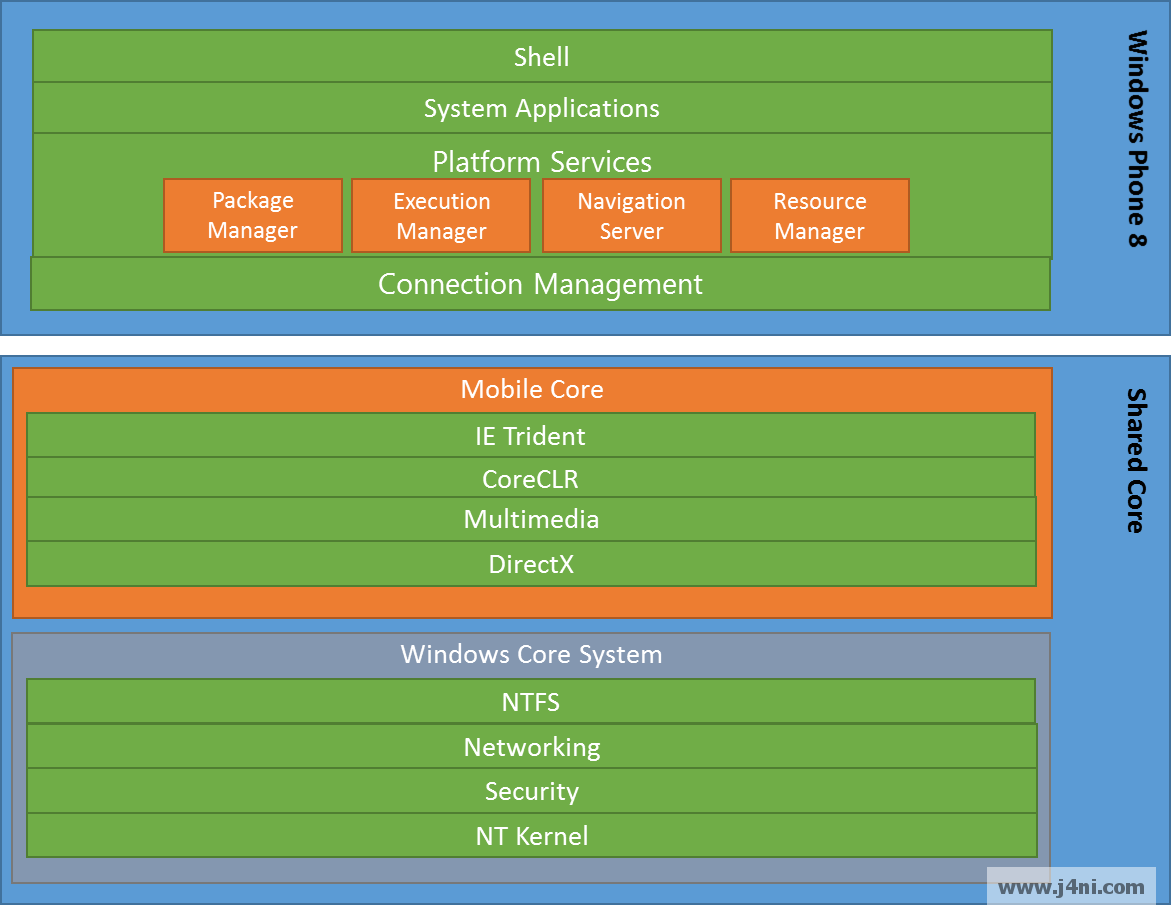
\includegraphics[width=1.0\textwidth]{WP8Architecture.png}
\caption{Architektura systému Windows Phone 8 \cite{wp8_kernel_architecture}}
\label{fig:WP8Architecture}
\end{figure}

Na obrázku \ref{fig:WP8Architecture} vidíme sdílenou část jádra nazvanou „Windows Core System“. Jedná se o klíčovou část jádra systému Windows Phone a nachází se zde nejdůležitější systémové funkce, jako je podpora NTFS filesystému, bezpečnostní funkce, podpora pro síťování apod \cite{wp8_kernel_architecture}. 

Sekce nazvaná „Mobile Core“ obsahuje také značnou část kódu sdílenou s dospělými Windows, nicméně je již mírně modifikovaná pro mobilní použití \cite{wp8_kernel_architecture}. V této části jádra se nachází například srdce internetové prohlížeče Trident, podpora pro přehrávání mutlimédií a podobně.

Nad jádrem se nachází vrstva se systémovými aplikacemi, jako je People Hub, přehrávač hudby a videa, dále vrstva Windows Phone Shell, Connection Management a tzv. Platform Services. Volání z této vrstvy využívají všechny uživatelské aplikace. Nachází se zde například Package manager, který se stará o celý životní cyklus aplikace od nainstalování po její odstranění. Dále zde najdeme Resource manager, který sleduje jaká aplikace využívá které systémové prostředky a do jaké míry \cite{wp8_kernel_architecture}. V případě problémů může „neposlušnou“ aplikaci ukončit.

\subsection{Aplikační technologie}
U předchozí verze Windows Phone si uživatelé často stěžovali na dlouhou prodlevu při spouštění aplikací. To bylo zapříčiněno především způsobem kompilace, který byl použit. Aplikace se zkompilovávala za běhu znovu a znovu podle toho, jaké funkce uživatel používal \cite{wp8_compile_cloud}. Tento postup byl příčinou často pomalých a těžkopádných aplikací.

U nové verze systému se Microsoft pokusil tento problém vyřešit. Zvolil metodu, kterou nazývá „Compile in the Cloud“. Průběh celého procesu je vidět na obrázku \ref{fig:WP8Compilation}. 

\begin{enumerate}
	\item Vývojář zkompiluje aplikaci pomocí C\# překladače a ta se přeloží do mezijazyka.
	\item Tento obraz nahraje do Windows Phone Store, kde je v průběhu nahrávání zkompilován MDIL překladačem do dalšího mezijazyka – Machine Dependent Intermediate Language.
	\item Uživatel si stáhne obraz aplikace právě v kódu MDIL.
	\item Linker při každém spuštění aplikace ověří závislosti a dovede převod do finálního strojového kódu.
\end{enumerate}

V čem je výhoda tohoto řešení? Mezijazyk MDIL je velmi podobný finálnímu strojovému kódu. Zásadní odlišností je nahrazení některých potenciálně rizikových částí symboly, které jsou doplněny až při slinkování finální aplikace \cite{wp8_compile_cloud}. Například při aktualizaci telefonu mohou být porušeny některé závislosti, na kterých aplikace závisí. Při jejím spuštění to však Linker snadno odhalí a aktualizuje příslušné části nativního kódu.

Aplikace samotná pak běží jako samostatný proces, který se může necházet v několika stavech: 1. běžící, 2. spící, 3. tombstone (zombie).

\begin{figure}\centering
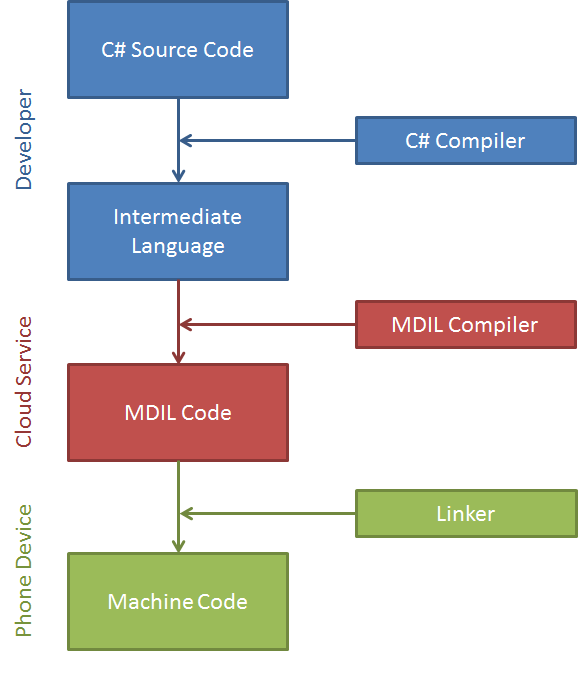
\includegraphics[width=1.0\textwidth]{wp8_cloud_compilation.png}
\caption{Průběh sestavení aplikace pro systém Windows Phone 8 \cite{wp8_compile_cloud}}
\label{fig:WP8Compilation}
\end{figure}

\subsection{Vývojářské technologie}
Pro vývoj aplikací pro systém Windows Phone 8 (ale i pro desktopové Windows) se primárně používá jazyk C\#. Tento jazyk byl vyvinutý spolu s frameworkem .NET firmou Microsoft. C\# je objektově orientovaný jazyk, u jehož syntaxe se Microsoft inspiroval u programovacích jazyků z rodiny C. Některé aspekty však přejal také z oblíbené Javy.

Framework .NET je komplexní balík knihoven a rozhraní určených pro vývoj, kompilaci a spouštění aplikací pro platformu Windows.

\subsection{Vývojářské nástroje}
Také pro platformu Windows Phone 8 existuje balík nástrojů určený pro vývoj nativních aplikací – Windows Phone 8 SDK. Jeho součástí je odlehčená verze Microsoft Visual Studia – Visual Studio Express 2012. Visual Studio je velmi oblíbené vývojové prostředí s širokým spektrem funkcí, jež sou vývojářům k dispozici. SDK obsahuje množství nástrojů pro návrh, testování, debugování a emulátory pro běh uživatelských aplikací.

\section{Platforma Firefox OS} \label{Sec:FxOS}
\subsection{Systémová architektura}
Jak můžeme vidět na obrázku \ref{fig:FxOSArchitecture}, architekturu platformy Firefox OS můžeme rozdělit do tří hlavních vrstev \cite{fxOs_architecture}.

\begin{enumerate}
	\item Gonk je nejnižší vrstva systému. Jeho součástí je jádro operačního systému Linux, které se stará o komunikaci s hardwarem zařízení. Dále v této vrstvě najdeme open-source knihovny pro práci s USB (libusb), pro komunikaci pomocí Bluetooth a podobně. Některé knihovny jsou dokonce přejaté z operačního systému Android (GPS, fotoaparát atd.) \cite{fxOs_architecture}. Můžeme zjednodušeně říci, že Gonk je distribucí operačního systému Linux.
	\item Gecko není jen jádrem prohlížeče Firefox, ale i srdcem systému Firefox OS. Ve Firefox OS nalezneme Gecko portované speciálně pro „distribuci“ Gonk. Gecko přináší podporu pro základní webové technologie (HTML, CSS, JavaScript), které vývojáři používají pro vývoj nativních aplikací pro systém Firefox OS. Součástí této vrstvy je i řada otevřených standardů WebAPI, na jejichž vývoji pracuje společnost Mozilla. Jejich cílem je standardizovat (W3C) webová volání, jež budou poskytovat jednotný přístup vývojářům webových mobilních aplikací (a dokonce i obyčejných webových stránek) k hardwarovému vybavení telefonu. Součástí tohoto WebAPI je již celá řada volání, které vývojáři používají při vývoji svých aplikací pro Firefox OS. Patří mezi ně například volání na ovládání Geolokace, Kontaktů, Fotoaparátu a podobně. Více o WebAPI si řekneme v kapitole XY. % TODO ověřit
	\item Gaia je nejvyšší vrstvou systému Firefox OS. Gaia má na starost vše okolo zobrazování uživatelského rozhraní. Domovská obrazovka, lock screen a všechny systémové aplikace jsou vytvořeny a spravovány právě pomocí Gaii. Samotná Gaia je v duchu filozofie systému Firefox OS napsaná čistě v HTML, CSS a JavaScriptu \cite{fxOs_architecture}. Uživatelské aplikace se instalují vedle této vrstvy.
\end{enumerate}

\begin{figure}\centering
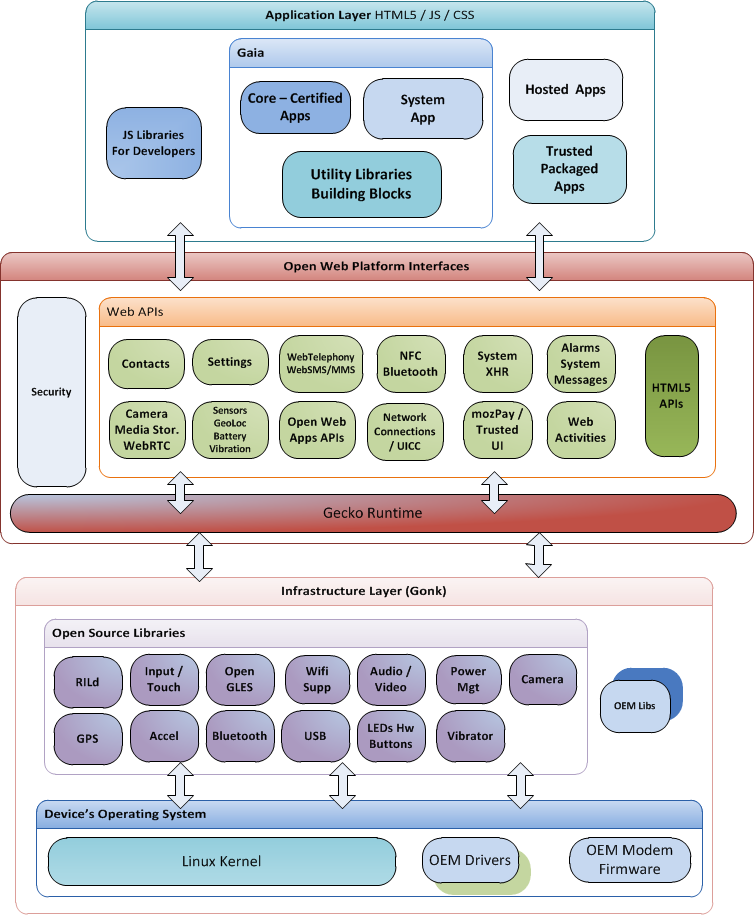
\includegraphics[width=1.0\textwidth]{FirefoxOS_architecture.png}
\caption{Architektura systému Firefox OS \cite{fxOs_architecture}}
\label{fig:FxOSArchitecture}
\end{figure}

\subsection{Aplikační technologie}
Protože nativní aplikace pro systém Firefox OS není nic jiného než „trochu vylepšená“ webová stránka (přesněji tzv. Open Web App \cite{faqs_mozilla}), nemůžeme od Firefox OS očekávat jakýkoliv proces kompilace.

Taková webová aplikace může samozřejmě fungovat jako běžná webová stránka uvnitř internetového prohlížeče. Uživatelé ovšem obvykle očekávají od mobilní aplikace více než od webové stránky. Aplikace ve Firefox OS běží mimo internetový prohlížeč. Ke svému běhu využívají tzv. Web runtime. Web runtime je software obsažený v internetovém prohlížeči, který však může běžet samostatně a zajišťuje celý životní cyklus aplikace od jejího spuštění, po obsluhu jejích požadavků až po její ukončení uživatelem \cite{apps_architecture}.

\subsection{Vývojářské technologie}
Jelikož jsme již naznačili, že pro vývoj nativních aplikací pro Firefox OS se používají pouze webové technologie dnes souhrnně (nesprávně?) označované jako rodina HTML5, do kterých řadíme:

\begin{enumerate}
	\item HTML5 jako značkovací jazyk ve své páté (dosud neoficiální) verzi obohacen o mnohé moderní funkce jako je geolokace, lokální databáze či nativní podpora pro přehrávání videa a audia.
	\item CSS3 pro definici vzhledu a částečně i chování uživatelského rozhraní aplikace.
	\item JavaScript je interpretovaný programovací jazyk, který se používá pro zajištění aplikační logiky. Jeho syntaxe se inspirovala u programovacích jazyků C/C++ a Java.
\end{enumerate}

\subsection{Vývojářské nástroje}
Mozilla nenabízí vývojářům aplikací pro Firefox OS (který stále ještě není v oficiálním prodeji) žádný balík se vším potřebným jako je tomu u jiných platforem. Důvodem pro tento fakt je pravděpodobně všudypřítomnost vývojářských nástrojů pro webové stránky/aplikace.

Přesto však firma Mozilla na konci roku 2012 vydala emulátor systému Firefox OS, na kterém mohou vývojáři testovat své aplikace aniž by museli vlastnit reálné zařízení. Firefox OS Simulator existuje pro Windows, Mac i Linux a lze jej dokonce získat i jako plugin do desktopové verze internetového prohlížeče Firefox \cite{announcing_fxOS_simulator}.